% \begin{table}[t] 
% % \begin{wraptable}{R}{0.5\linewidth}
% \caption{
% % The Performance (\texttt{Pass@1}, \texttt{Pass@10}, and \texttt{Pass@100}) comparison of LLMs for code generation on HumanEval benchmark. For the model with various model size, we only report the largest size version of each model.
% \revise{The performance comparison of LLMs for code generation on the HumanEval \cite{chen2021evaluating} benchmark, measured by \texttt{Pass@1}. 
% % Due to the limitations of computational resources we faced, we directly cite the experimental results from the original papers or widely recognized open-source leaderboard in research community.
% For models with various sizes, we report only the largest size version of each model with the magnitude of \texttt{B} parameters. $^\ddag$ denotes instruction-tuned models.
% % DeepSeek-Coder-V2-Instruct is an open-source Mixture-of-Experts (MoE) code language
% % model, which has 236B parameters with only 21B activation parameters. 
% } 
% }
% \label{tab:performance_bigcodebench}
% \centering
% \scalebox{0.82}{
% \rotatebox{0}{
%     \begin{tabular}{clrc}
%     \toprule
%     & \textbf{Model} & \textbf{Size} & \texttt{Full pass@1} \\ 
% \midrule
%     \multirow{10}{*}{\textbf{Closed Source}} 
%          & GPT-4o-0513 \cite{gpt-4o} & - & 51.1 \\
%          & GPT-4-Turbo-0409 \cite{gpt-4-turbo} & - & 48.2 \\
%          & GPT-4-0613 \cite{achiam2023gpt}& - & 46  \\
%          & GPT-3.5-Turbo-0125 \cite{gpt-3.5-turbo}& - & 39.1 \\
%          & Claude-3.5-Sonnet \cite{claude3} & - & 46.8 \\
%          & Claude-3-Opus \cite{claude3} & - & 45.5 \\
%          & Claude-3-Sonnet \cite{claude3} & - & 42.7 \\
%          & Claude-3-Haiku \cite{claude3} & - & 39.4 \\
%          & Gemini-1.5-Pro \cite{reid2024gemini} & - & 43.8 \\
%          & Gemini-1.5-Flash \cite{reid2024gemini} & - & 43.5 \\
%          \midrule
%     \multirow{11}{*}{\textbf{Open Source}} 
%          & $^\ddag$Codestral \cite{codestral} & 22B & 41.8 \\
%          & $^\ddag$DeepSeek-Coder-V2-Instruct \cite{zhu2024deepseek}  & 21B (236B) & 48.2 \\
%          & $^\ddag$Qwen2.5-Coder-Instruct \cite{hui2024qwen2} & 7B & 40.4 \\
%          & $^\ddag$StarCoder2-Instruct \cite{starcoder2instruct} &  15.5B  & 37.6 \\
%          & $^\ddag$CodeGemma-Instruct \cite{codegemma_2024}  & 7B  & 32.3 \\
%          & $^\ddag$WaveCoder-Ultra \cite{yu2023wavecoder} & 6.7B & 33.9 \\
%          & $^\ddag$CodeQwen1.5-Chat \cite{codeqwen} & 7B & 39.6 \\
%          & $^\ddag$Magicoder-S-DS \cite{wei2023magicoder} & 7B & 36.2 \\
%          & $^\ddag$DeepSeek-Coder-Instruct \cite{guo2024deepseek} & 33B & 42 \\
%          & $^\ddag$Phi-3-Medium-128K-Instruct \cite{abdin2024phi} & 14B & 36.8 \\
%          & $^\ddag$Code Llama-Instruct \cite{roziere2023code} & 70B & 40.7 \\
%          & $^\ddag$CodeGeeX4 \cite{zheng2023codegeex} & 9B & 40 \\
%     \bottomrule
%     \end{tabular}
% }
% }
% \vspace{-10pt}
% % \end{wraptable}
% \end{table}

\begin{figure*}[t]
\centering
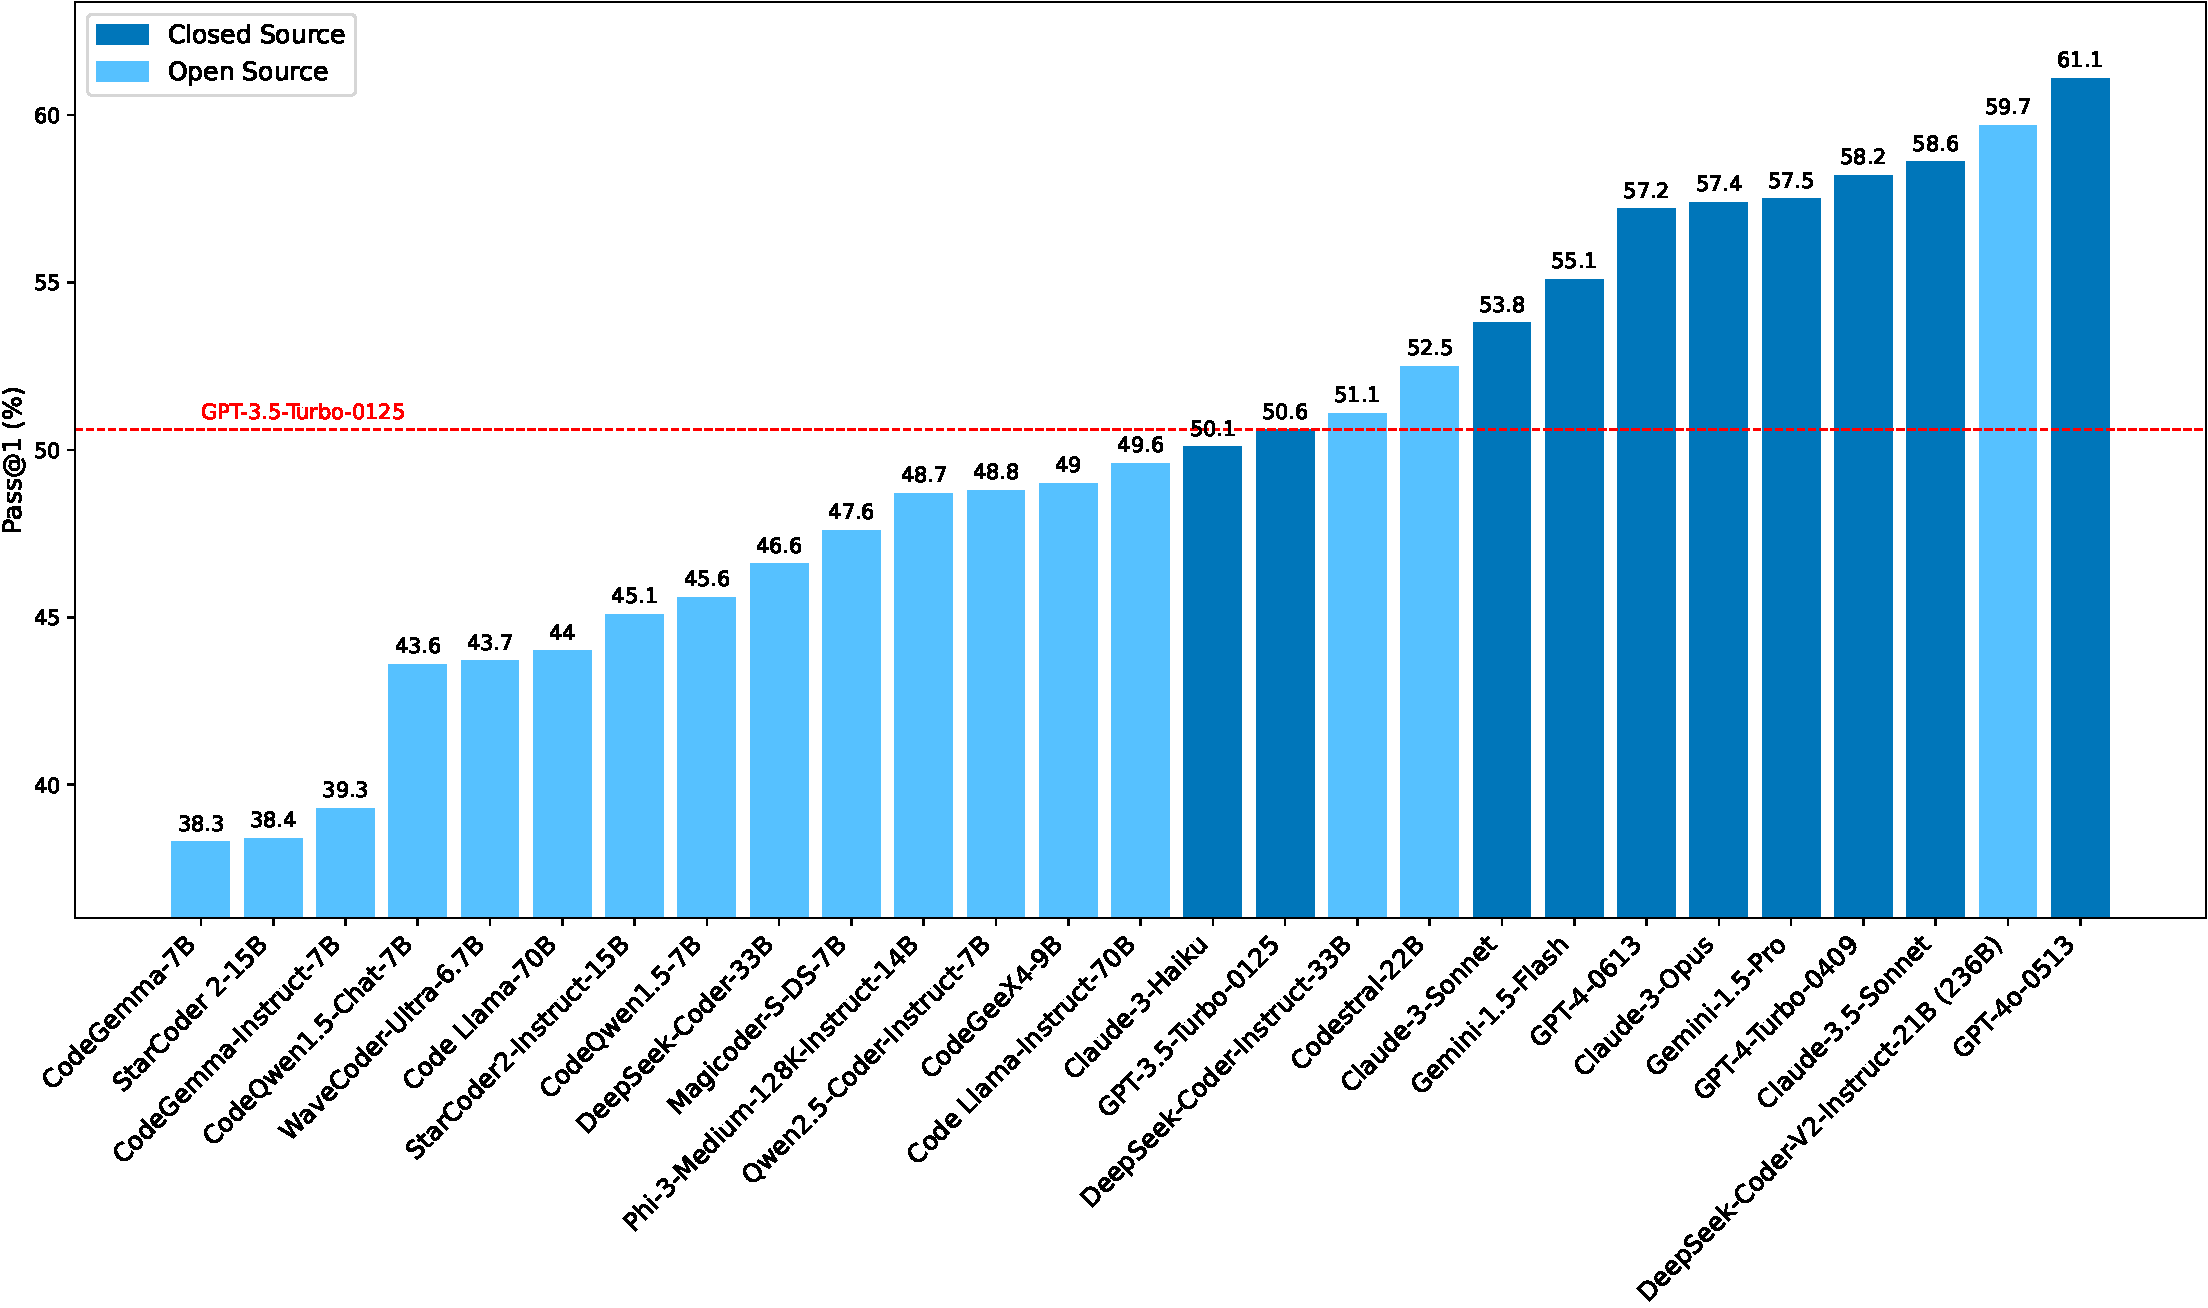
\includegraphics[width=\linewidth]{images/bigcodebench_complete_bar.pdf}
\caption{\done{The performance comparison of LLMs for code generation on the BigCodeBench \cite{zhuo2024bigcodebench} benchmark, measured by \texttt{Pass@1}. For models with various sizes, we report only the largest size version of each model with a magnitude of \texttt{B} parameters.} 
}
\label{fig:bigcodebench_performance}
\end{figure*}